\section{Computation}

\begin{frame}{1-D discrete case}
    \footnotesize
    Here $\mX=\mY=\R$. Suppose
     $\alpha=\frac{1}{n}\sum_{i=1}^n \delta_{x_i}$
    and $\beta=\frac{1}{n}\sum_{i=1}^n \delta_{y_i}$
    where $x_1\leq \cdots \leq x_n$ and $y_1\leq \cdots \leq y_n$.

    \begin{figure}
        \centering
        \captionsetup{font=scriptsize}
        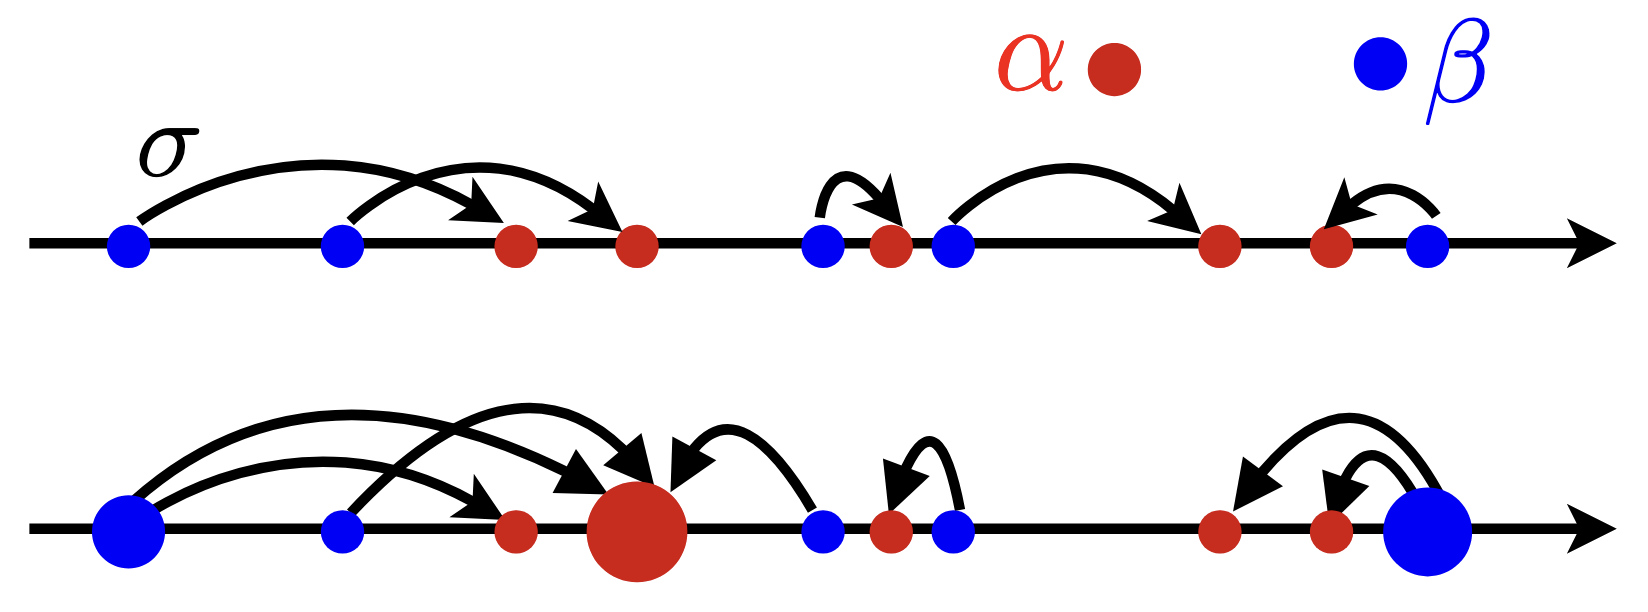
\includegraphics[width=0.5\textwidth]{png/1d-discrete.png}
        \caption{1-D optimal transport in discrete case}
    \end{figure}
    
    Then the $p$-Wasserstein distance can be simply computed by
    \begin{equation}
        \wass_p(\alpha,\beta)^p = \frac{1}{n}\sum_{i=1}^n |x_i-y_i|^p.
    \end{equation}
    It's in fact a greedy algorithm.
\end{frame}